\documentclass[a4paper,12pt]{article}
%\documentclass[a4paper,10pt]{scrartcl}

\usepackage[utf8x]{inputenc}
\usepackage{amsfonts}
\usepackage{amsmath,esint}
\usepackage{graphicx}
\usepackage{pdfpages}
\usepackage{sansmath}
\usepackage{hyperref}
\usepackage{natbib}

\usepackage{tikz}


\definecolor{boiseBlue} {RGB}{29,72,159}
\definecolor{rojoAmor} {RGB}{171,13,4}
\definecolor{moradoAmor} {RGB}{93,8,113}
\definecolor{verdeAmor} {RGB}{98,158,31}
\definecolor{negro} {RGB}{10,10,10}
\definecolor{lgreen} {RGB}{180,210,100}
\definecolor{dblue}  {RGB}{20,66,129}
\definecolor{ddblue} {RGB}{11,36,69}
\definecolor{lred}   {RGB}{220,0,0}
\definecolor{nred}   {RGB}{224,0,0}
\definecolor{norange}{RGB}{230,120,20}
\definecolor{nyellow}{RGB}{255,221,0}
\definecolor{ngreen} {RGB}{98,158,31}
\definecolor{dgreen} {RGB}{78,138,21}
\definecolor{nblue}  {RGB}{28,130,185}
\definecolor{jblue}  {RGB}{20,50,100}

\usepackage{listings}
\usepackage{xcolor}
\lstset{language=C++,
		basicstyle=\ttfamily,
	       backgroundcolor=\color{black!5}\ttfamily,
                keywordstyle=\color{nblue}\ttfamily,
                stringstyle=\color{nred}\ttfamily,
                commentstyle=\color{ngreen}\ttfamily,
                morecomment=[l][\color{moradoAmor}]{\#}
}

\newenvironment{rcases}{\Big.\begin{aligned}}{\end{aligned}\Big\rbrace}

\renewcommand{\familydefault}{\sfdefault}
\renewcommand{\labelitemii}{$\circ$}

\newcommand{\specialcell}[2][c]{%
  \begin{tabular}[#1]{@{}c@{}}#2\end{tabular}}
% \specialcell{Foo\\bar}

\title{\Huge{
\color{nblue}g\color{nred}er\color{ngreen}j\color{nblue}o\color{nred}i\color{moradoAmor}i}
\color{black}\\ Imaging using DC currents \\ \small{summer 2017}}
\author{}
\date{}

\pdfinfo{%
  /Title    ()
  /Author   ()
  /Creator  ()
  /Producer ()
  /Subject  ()
  /Keywords ()
}

\begin{document}
\maketitle
%-------------------
% fwd
%-------------------
\section{Forward}
Using the finite volume method, solve for $\varphi$ the DC process
\[
-\nabla\cdot\sigma\nabla \varphi = s 
\]
over a rectangular region $\Omega$ (simulating a slice in depth of the earth) with Neumann boundary 
conditions on one edge, and Robin boundary conditions over the rest. Sources are assumed to be on the 
air-ground interface.
\begin{figure}
\centering
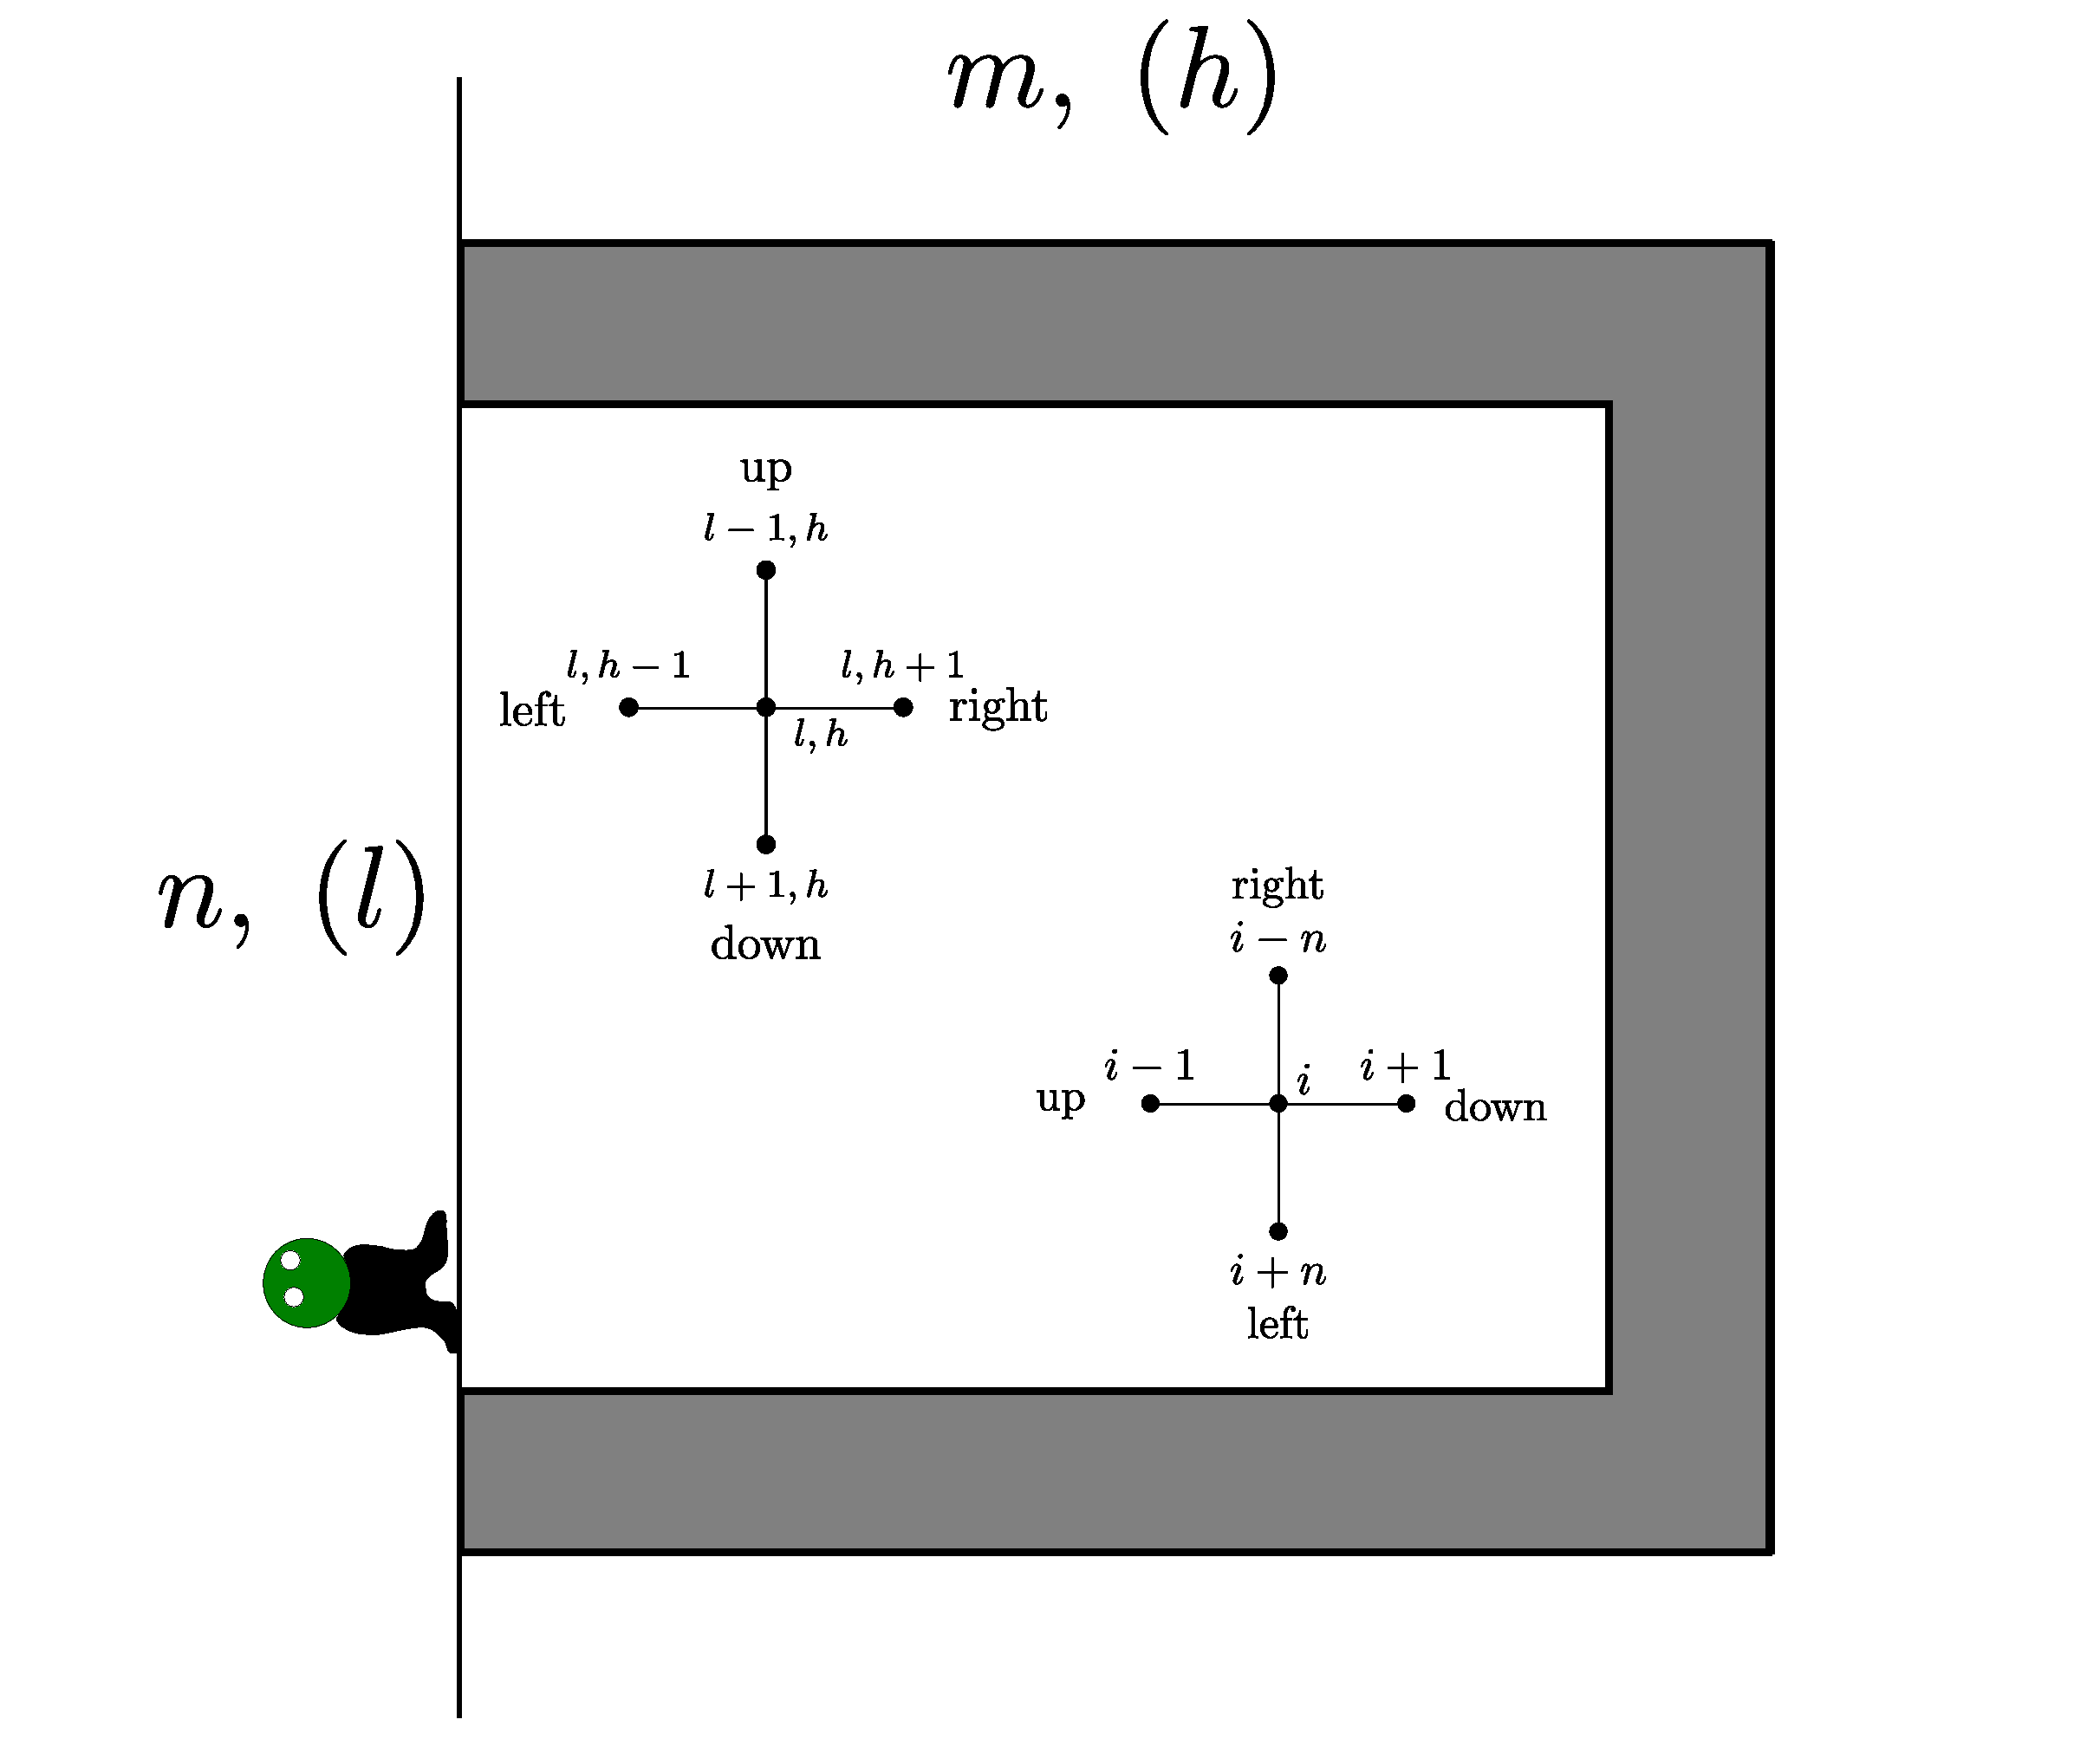
\includegraphics[width=0.8\textwidth]{../pics/tikz/svg/domain.pdf} 
\caption{Computational domain of $\Omega$. Orientation is {\it matrix} orientation. 
Different {\it up, right, down, left} depending on wether node is written in $[l,h]$ (matrix notation), 
or if it is written as index $i$ (vector notation). The air-ground interface is where the black dude is. 
Gray area is where Robin b.c. take place.}
\end{figure}
%
\begin{figure}
\centering
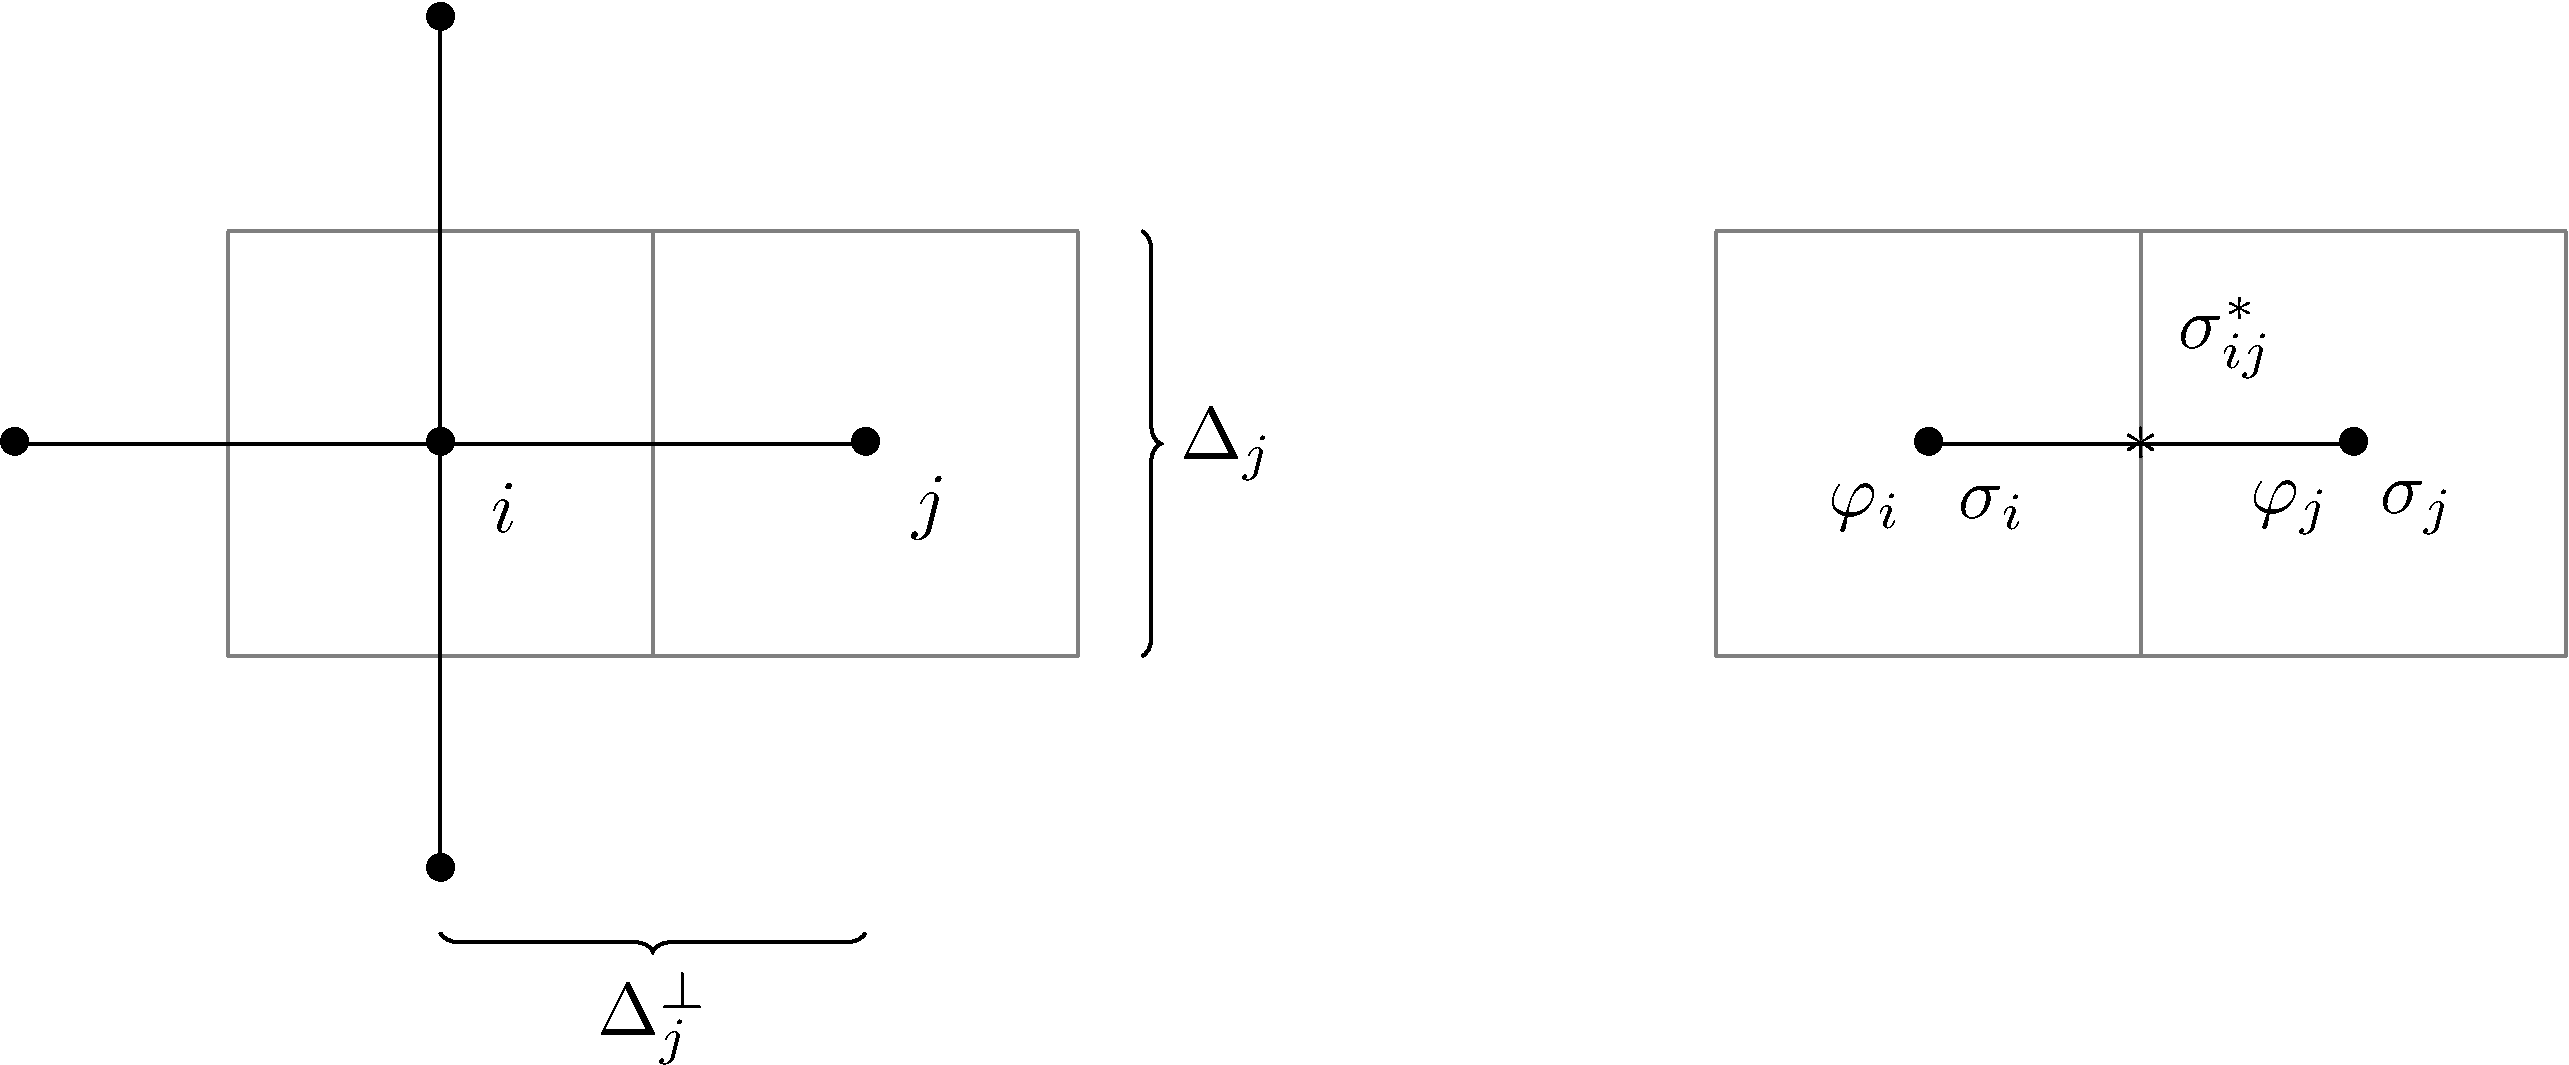
\includegraphics[width=0.8\textwidth]{../pics/tikz/svg/regions.pdf} 
\caption{Regions inside $\Omega$.}
\end{figure}
%
\begin{itemize}
\item Give grid size $n,m$.
\item Build $\sigma$. ($n\times m$ matrix)
\item Build source $s$. ($nm\times 1$ vector)
\item Build observation matrix $M$. ($d\times nm$ matrix)
\item Build grid edge lengths $\Delta$. (two $n\times m$ matrices)
\item Build boundary condition smoothers $\alpha=\alpha(s,\Delta)$. ($n\times m$ matrix) 
\item Build matrix $L=L(\sigma,\Delta,\alpha)$, b.c. are included. ($nm\times nm$ matrix)
\item Compute $\varphi=L^{-1}s$. ($nm\times 1$ vector)
\item Compute observations (data) $d = M\varphi$. ($d\times 1$ vector)
\end{itemize}
Matrix and vector form for writing the grid will be used interchangeably. Typically $[l,h]$ will refer to matrix 
form, and $i$ or $j$ to vector form.
%-------------------
% inverse
%-------------------
\section{Inverse}
Given data $d^o$, find $\sigma\approx\sigma^o$ that under the forward model recreates 
$d(\sigma)\approx d^o$. 
This is done by optimizing
\begin{align*}
{\sf E}(\sigma;\,d^o) &= \sum_i \frac{e_i^2}{2} & e = d-d^o,
\end{align*}
with respect to $\sigma$.
\begin{itemize}
\item Build $\sigma^o$.
\item Compute $d^o$.
\item Introduce noise on $d^o$.
\item Perform optimizing algorithm on ${\sf E}$.
\end{itemize}
%-------------------
% file names
%-------------------
\section{File names}
{\bf Constructors}
\begin{itemize}
\item \texttt{dc\_sigma.m} builds $\sigma$.
\item \texttt{dc\_sosi.m} builds $s_+,\, s_-$ in vector form.
\begin{itemize}
 \item \texttt{dc\_sosi\_compact.m} builds $s_+,\, s_-$ in index form.
\end{itemize}
\item \texttt{alphas.m} builds $\alpha$.
\item \texttt{dc\_L.m} builds $L$.
\item \texttt{dc\_M.m} builds $M$.
\item \texttt{dc\_S.m} builds $S$.
\end{itemize}
{\bf Procedures}
\begin{itemize}
\item \texttt{dc\_fwd.m} computes $\varphi,e,L$.
\item \texttt{dc\_adj.m} computes adjoint $\lambda$.
\item \texttt{dc\_Jte.m} computes jacobian-transposed of $\varphi$ times a vector.
\item \texttt{dc\_Jg.m} computes jacobian of $\varphi$ times a vector.
\item \texttt{dc\_gd.m} performs gradient descent on ${\sf E}$.
\item \texttt{dc\_bfgs.m} perfroms BFGS on ${\sf E}$.
\item \texttt{dc\_armijo.m} computes simple back-track line search on ${\sf E}$.
\item \texttt{dc\_gd\_stoch.m} performs stochastic gradient descent on ${\sf E} = \sum_i{\sf E}_i$.
\end{itemize}
{\bf Examples}
\begin{itemize}
 \item \texttt{dc\_run.m}
\item \texttt{dc\_run\_many.m}
\item \texttt{dc\_inv.m}
\item \texttt{dc\_inv\_many.m}
\end{itemize}
%-------------------
% L
%-------------------
\newpage
\section{Building $L$}
We want to discretize
\begin{align*}
L_{dc} \approx \underbrace{-\nabla\cdot\sigma\nabla}_{\mathcal{L}_{dc}}
\end{align*}
\begin{align*}
L_{i,:} &=  
\Big[
\underbrace{ 
a_{ik}\cdot\sigma_i +
\sum_j a_{ij}\cdot\sigma_{ij}^{*}
}_{i'th \text{ entry}}
\hspace{4em}
\underbrace{ 
-b_{ij}\cdot\sigma_{ij}^{*}
}_{j'th \text{ entries}}
\Big],
&
\sigma_{ij}^{*} = \frac{2\sigma_i\sigma_j}{\sigma_i+\sigma_j}
\end{align*}
where,
\begin{align*}
b_{ij} &=
\frac{\Delta_j}{\Delta_{j}^{\bot}} & \text{for all nodes} \\
a_{ij} &=
\frac{\Delta_j}{\Delta_{j}^{\bot}} & \text{inner nodes \& Neu nodes} \\
a_{ik} &=
\Delta_{k_i} \cdot \alpha_{ik}
 & \text{Robin nodes ($0$ otherwise)} \\
 a_{ik} &=
 \Delta_{k_1} \cdot c_{1} + \Delta_{k_2} \cdot c_{2}
 & \text{corner nodes ($0$ otherwise)} \\
\end{align*}
Different planes of $\Delta$
\begin{align*}
\Delta_{:,:,1} & \text{ VERTICAL edges} & \text{ of node }(:,:) \\
\Delta_{:,:,2} & \text{ HORIZONTAL edges} & \text{ of node }(:,:)
\end{align*}
%
Different planes of $LL$:
\begin{align*}
LL_{:,:,1} & \text{ entries for $L$ of DOWN} & \text{ neighbor of }(:,:) \\
LL_{:,:,2} & \text{ entries for $L$ of UP} & \text{ neighbor of }(:,:) \\
LL_{:,:,3} & \text{ entries for $L$ of RIGHT} & \text{ neighbor of }(:,:) \\
LL_{:,:,4} & \text{ entries for $L$ of LEFT} & \text{ neighbor of }(:,:) \\
LL_{:,:,5} & \text{ entries for $L$ of GHOST} & \text{ neighbor of }(:,:) \\
LL_{:,:,6} & \text{ entries for $L$ of $-$STACK of} & \text{ all neighbors of }(:,:)
\end{align*}
Vertical (down) neighbor
\begin{align*}
LL_{l,h,1} =&
 -2\frac{\sigma_{l,h} \odot \sigma_{l+1,h} }	{\sigma_{l,h} + \sigma_{l+1,h}} \; \odot \;
 \frac{\Delta_{l,h,2} + \Delta_{l,h+1,2} } {2\Delta_{l+1,h,1} }.
\end{align*}
%
Vertical (up) neighbor
\begin{align*}
LL_{l,h,2} =&
 -2 \frac{ \sigma_{l,h} \odot \sigma_{l-1,h} }{\sigma_{l,h} + \sigma_{l-1,h}} \; \odot \;
 \frac{\Delta_{l,h,2} + \Delta_{l,h+1,2}} {2\Delta_{l,h,1} }.
\end{align*}
%
Horizontal (right) neighbor
\begin{align*}
LL_{l,h,3} =&
-2 \frac{ \sigma_{l,h} \odot \sigma_{l,h+1}} {\sigma_{l,h} + \sigma_{l,h+1}} \; \odot \;
\frac{ \Delta_{l,h,1} + \Delta_{l+1,h,1} } {2\Delta_{l,h+1,2} }.
\end{align*}
%
Horizontal (left) neighbor
\begin{align*}
LL_{l,h,4} =&
-2 \frac{ \sigma_{l,h} \odot \sigma_{l,h-1} } {\sigma_{l,h} + \sigma_{l,h-1}} \; \odot \;
\frac{ \Delta_{l,h,1} + \Delta_{l+1,h,1}}{2\Delta_{l,h,2}}.
\end{align*}
%
%   ghosts
% 
Ghost up
\begin{align*}
LL_{1,h,5} =&
-\sigma_{1,h} \; \odot \;
\frac{ \Delta_{1,h,2} + \Delta_{1,h+1,2}}{2}  \; \odot \;
\alpha_{1,h}.
\end{align*}
Ghost right
\begin{align*}
LL_{l,m,5} =&
-\sigma_{l,m}  \; \odot \;
\frac{ \Delta_{l,m,1} + \Delta_{l+1,m,1}}{2}  \; \odot \;
\alpha_{1,m}.
\end{align*}
Ghost down
\begin{align*}
LL_{n,h,5} =&
-\sigma_{n,h}  \; \odot \;
\frac{ \Delta_{n,h,2} + \Delta_{n,1,2}}{2}  \; \odot \;
\alpha_{n,h}.
\end{align*}
%
% corners
%
Corner 3 up
\begin{align*}
LL_{1,m,5} =&
-\sigma_{1,m} \; \odot \;
\frac{ \Delta_{1,m,2} + \Delta_{1,1,2}}{2}  \; \odot \;
c_{1,1}.
\end{align*}
Corner 3 right
\begin{align*}
LL_{1,m,5} =& LL_{1,m,5}
-\sigma_{1,m} \; \odot \;
\frac{ \Delta_{1,m,1} + \Delta_{2,m,1}}{2}  \; \odot \;
c_{2,1}.
\end{align*}
Corner 4 down
\begin{align*}
LL_{n,m,5} =&
-\sigma_{n,m} \; \odot \;
\frac{ \Delta_{n,m,2} + \Delta_{n,1,2}}{2}  \; \odot \;
c_{1,2}.
\end{align*}
Corner 4 right
\begin{align*}
LL_{n,m,5} =& LL_{n,m,5} 
-\sigma_{n,m} \; \odot \;
\frac{ \Delta_{n,m,1} + \Delta_{1,m,1}}{2}  \; \odot \;
c_{2,2}.
\end{align*}
%-------------------
% S
%-------------------
\newpage
\section{Building $S$}
We want to discretize $S$ where,
\begin{align*}
-({\rm d}_{\sigma} \mathcal{L}_{dc}) \varphi \approx
-(\nabla_{\sigma}L_{dc})\varphi = S^t.
\end{align*}
Let $\partial_{\sigma_i}:=\partial_i$,
\[
\partial_i(\sigma_{ij}^{*}) = \frac{2 \sigma_{j}^{2}}{(\sigma_{i}+\sigma_{j})^2}=
\partial_i(\sigma_{ji}^{*})
\]
\begin{align*}
S_{i,:} &=  
\Big[
\underbrace{ 
-a_{ik}\varphi_i + 
\sum_j ( b_{ij}\varphi_j - a_{ij}\varphi_i ) \cdot \partial_i(\sigma_{ij}^{*}) 
}_{i'th \text{ entry}}
\hspace{3em}
\underbrace{ 
( a_{ji}\varphi_i - b_{ji}\varphi_j ) \cdot \partial_i(\sigma_{ji}^{*}) 
}_{j'th \text{ entries}}
\Big]
\end{align*}
where,
\begin{align*}
b_{ij} &=
\frac{\Delta_j}{\Delta_{j}^{\bot}} & \text{for all nodes} \\
a_{ij} &=
\frac{\Delta_j}{\Delta_{j}^{\bot}} & \text{inner nodes \& Neu nodes} \\
a_{ik} &= 
\Delta_{k_i} \cdot \alpha_{ik}
 & \text{Robin nodes ($0$ otherwise)} \\
 a_{ik} &=
 \Delta_{k_1} \cdot c_{1} + \Delta_{k_2} \cdot c_{2}
 & \text{corner nodes ($0$ otherwise)} \\
\end{align*}
and
\begin{align*}
b_{ji} &= b_{ij} & \text{for all nodes} \\
% \frac{\Delta_i}{\Delta_{i}^{\bot}} & \text{for all nodes} \\
a_{ji} &= a_{ij} & \text{for all nodes}
% \frac{\Delta_i}{\Delta_{i}^{\bot}} & \text{for all nodes}
\end{align*}
%
\begin{itemize}
\item The $i$'th entry of $S_{i,:}$ has information from $L_{i,:}$.
\item The $j$'th entries of $S_{i,:}$ have information from $L_{j,:}$, where $j$ has $i$ as neighbor.
\item $S_{i,:}$ has as many $j$'th entries as $i$ is a neighbor of.
\end{itemize}
%
The structure of the code for building $S$ is very similar to that of $L$, so just one example for each case 
is enough. See Figure (\ref{fig:S}) for a cool diagram explaining the code flow.
\\\\
Vertical (down) neighbor
\begin{align*}
SB_{l,h,1} =&
 \frac{\Delta_{l,h,2} + \Delta_{l,h+1,2} } {2\Delta_{l+1,h,1} }  \; \odot \; 
 \varphi_{l+1,h} \\
SA_{l,h,1} =&
 \frac{\Delta_{l,h,2} + \Delta_{l,h+1,2} } {2\Delta_{l+1,h,1} }  \; \odot \; 
 \varphi_{l,h} \\
 SD_{l,h,1} =&
 2 \left (\frac{ \sigma_{l+1,h} }{\sigma_{l,h} + \sigma_{l+1,h}}\right)^2
\end{align*}
%
%   ghosts
% 
Ghost up
\begin{align*}
SR_{1,h} =&
\frac{ \Delta_{1,h,2} + \Delta_{1,h+1,2}}{2}  \; \odot \;
\alpha_{1,h} \; \odot \;
\varphi_{1,h}
\end{align*}
Corner up \& right
\begin{align*}
SR_{1,m} =&
\left(
\frac{ \Delta_{1,m,2} + \Delta_{1,1,2}}{2}  \; \odot \;
c_{1,1} 
\; + \;
\frac{ \Delta_{1,m,1} + \Delta_{2,m,1}}{2}  \; \odot \;
c_{2,1}
\right)
\; \odot \;
\varphi_{1,h}
\end{align*}
%
\begin{figure}[!h]
\centering
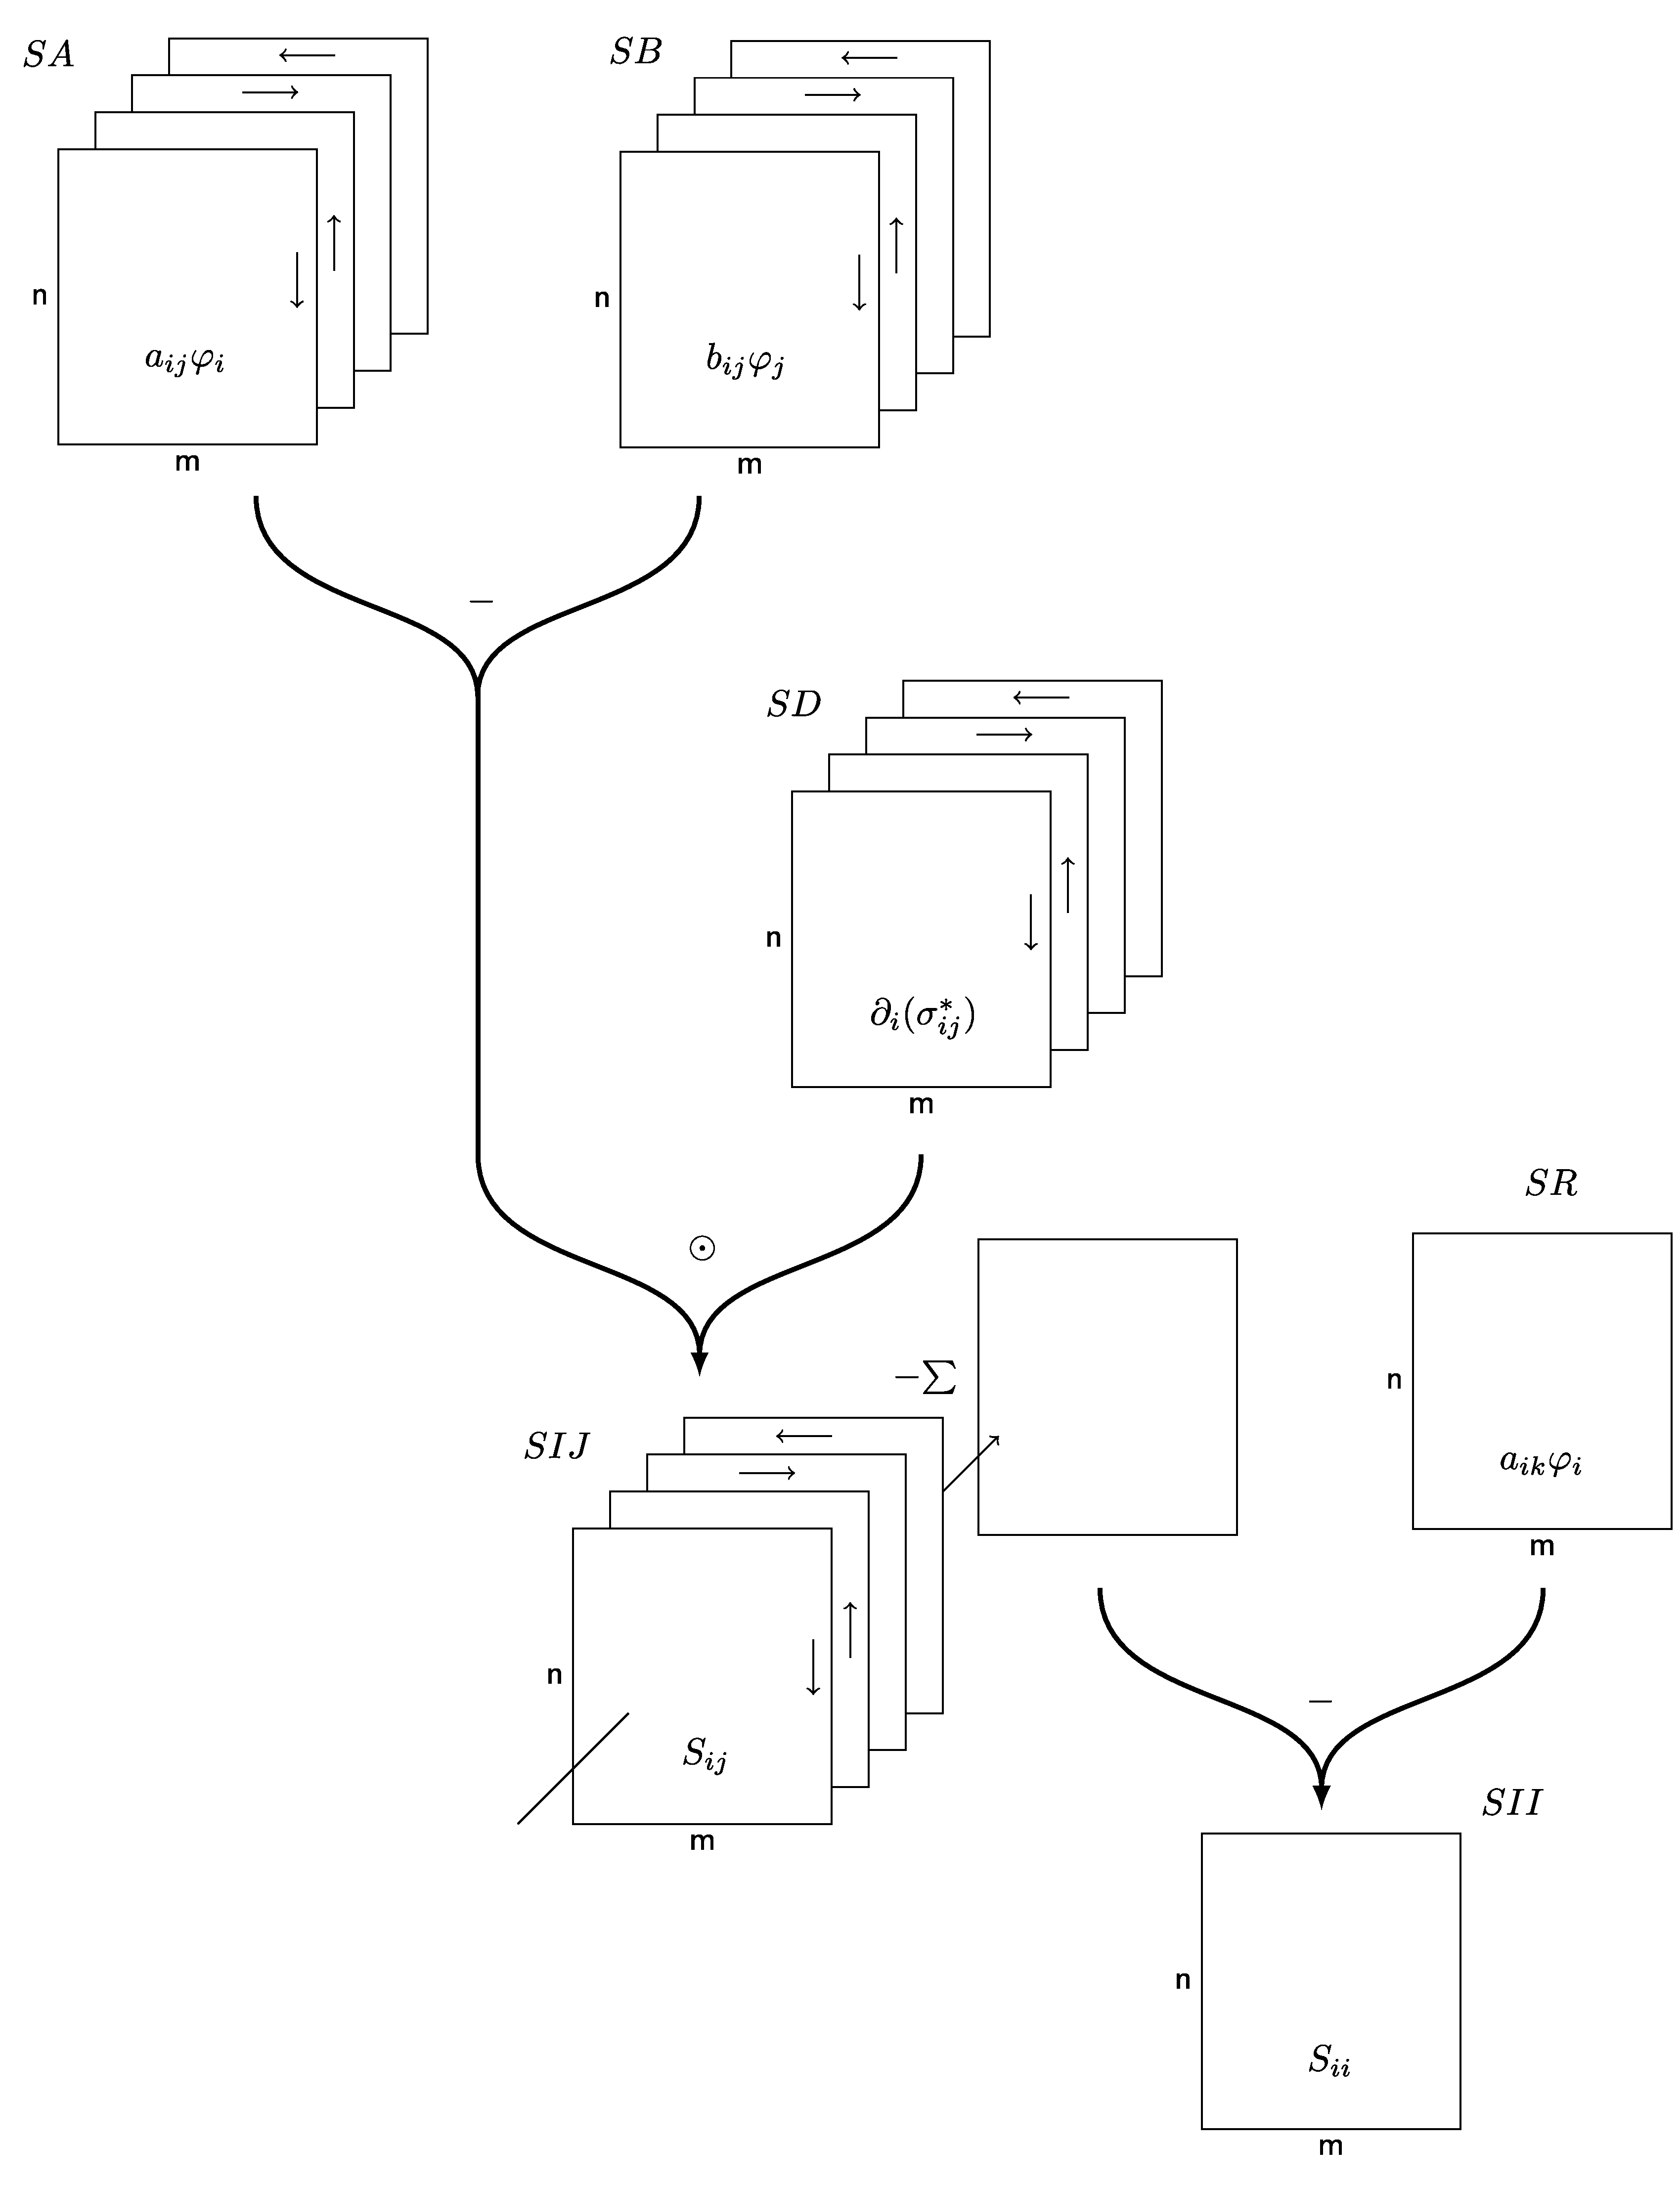
\includegraphics[width=1\textwidth]{../pics/tikz/svg/S.pdf} 
\caption{Building the entries of $S$. Matrices (and groups of) are labeled by their respective entry in the 
$i$'th node. Names used in the code are displayed next to the matrices.}
\label{fig:S}
\end{figure}
% --------------------------------------------------------------------------------------------
% 				real data
% --------------------------------------------------------------------------------------------
\section{Iris data - in}
Iris takes survey data in a \texttt{.txt} file with the format:
\begin{align}
\begin{matrix}
\text{r\#} & x & y & z \\
\vdots & \vdots & \vdots & \vdots \\
a & b & m & n \\
\vdots & \vdots & \vdots & \vdots \\
n_{sr}
\end{matrix}
\end{align}
where r\# is the electrode number, $(x,y,z)$ are its field coordinates, $(a,b,m,n)$ are source-receiver pairs and $n_{sr}$ is the number of source-receiver shots.
\\\\
See routine \texttt{dc\_gerjoii2iris.m} and script \texttt{gerjoii2iris\_dc.m}.
\\\\
\section{Iris data - out}
Iris performs experiments by picking a injecting current on the source and measuring on {\it some} of the receivers associated to that source, not all of them. The missing receivers for a given source are then covered with a different current magnitude.
\\\\
Routine \texttt{dc\_iris2gerjoii.m} and script \texttt{iris2gerjoii\_dc.m} bundle all common source shots in one cell type (\texttt{s\_i\_r\_d\_std$\{i_e\}$}) indexed by experiment number containing source, current, receivers, observed voltage and observed standard deviation. This bundle has sources and receivers in electrode number.
\\\\
To use the bundle \texttt{s\_i\_r\_d\_std$\{i_e\}$} in \color{nblue}g\color{nred}er\color{ngreen}j\color{nblue}o\color{nred}i\color{moradoAmor}i\color{black}\;the function \texttt{dc\_electrodes.m} converts numbered real coordinate electrodes into the vectorized format \texttt{dc\_fwd.m} needs:
\\\\
Here goes a receiver diagram: \\
rectangle of size $(n_{r}\times 2)$ labeled by columns $r_+,\,r_-$ and by rows $\#$ of receiver (these are the numbered receivers) $\to$ two rectangles each of size $(n_{r}\times 2)$ labeled by columns $x,\,z$, by rows $\#$ of receiver and one labeled $+$ and the other $-$ (these are the real coordinate receivers) $\to$ two rectangles each of size $(n_{r}\times 2)$ labeled by columns $ix,\,iz$, by rows $\#$ of receiver and one labeled $+$ and the other $-$ (these are the binned receivers). Then comes an arrow pointing down and an arrow pointing right, the down arrow goes to {\it expand to robin} and the right arrow goes to two rectangles each of size $(n_{r}\times 1)$ labeled $r_+,\,r_-$ and by rows $\#$ of receiver (these are the vectorized receivers).
\\\\
Here goes a source diagram: \\
rectangle of size $(1\times 2)$ labeled by columns $s_+,\,s_-$ (this is the numbered source) $\to$ two rectangles each of size $(1\times 2)$ labeled by columns $x,\,z$ and one labeled $+$ and the other $-$ (this is the real coordinate source) $\to$ two rectangles each of size $(1\times 2)$ labeled by columns $ix,\,iz$ and one labeled $+$ and the other $-$ (this is the binned source). Then comes an arrow pointing down and an arrow pointing right. The down arrow goes to {\it expand to robin}, then to the right $\to$ {\it clean source} and then up to two squares each of size $(1\times 1)$ labeled $s_+,\,s_-$ (this is the vectorized source). The right arrow goes to the vectorized source.
%
%------------
% biblio
%------------
%\newpage
%\bibliographystyle{plainnat}
%\bibliography{seis-flow}
%\nocite{*}
\end{document}